\documentclass[10pt,notes]{beamer}
\usecolortheme{whale}
\useinnertheme{rounded}
\useoutertheme{infolines}

\linespread{1.25}\selectfont
\beamertemplatenavigationsymbolsempty
\setbeamerfont{note title}{size=\tiny}
\setbeamertemplate{footline}[frame number]
\setbeamertemplate{itemize item}[triangle]
\setbeamertemplate{itemize subitem}[circle]
\setbeamertemplate{itemize subsubitem}[square]

\setbeamertemplate{headline}
{
  \leavevmode%
  \hbox{%
  \begin{beamercolorbox}[wd=.5\paperwidth,ht=2.5ex,dp=1.5ex,right,rightskip=1em]{section in head/foot}%
    \usebeamerfont{subsection in head/foot}\hspace*{2ex}\insertshorttitle
  \end{beamercolorbox}%
  \begin{beamercolorbox}[wd=.5\paperwidth,ht=2.5ex,dp=1.5ex,left,leftskip=1em]{subsection in head/foot}%
    \usebeamerfont{section in head/foot}\insertsectionhead\hspace*{2ex}
  \end{beamercolorbox}}%
  \vskip0pt%
}

\makeatletter
\setbeamertemplate{footline}
{
  \leavevmode%
  \hbox{%
  \begin{beamercolorbox}[wd=.925\paperwidth,ht=2.5ex,dp=1ex,center]{author in head/foot}%
    \usebeamerfont{author in head/foot}\insertshortauthor
  \end{beamercolorbox}%
  \begin{beamercolorbox}[wd=.075\paperwidth,ht=2.5ex,dp=1ex,right]{date in head/foot}%
    \insertframenumber{} / \inserttotalframenumber\hspace*{2ex} 
  \end{beamercolorbox}}%
  \vskip0pt%
}
\makeatother

\makeatletter
\defbeamertemplate*{note page}{infolines}
{%
  {%
    \usebeamerfont{note title}\usebeamercolor[fg]{note title}%
    \ifbeamercolorempty[bg]{note title}{}{%
      \insertvrule{.0325\paperheight}{note title.bg}%
      \vskip-.0325\paperheight%
      \nointerlineskip%
    }%
    \nointerlineskip
    \leavevmode
    \vbox to .0325\paperheight{\vfil
        \begin{minipage}[t]{.5\linewidth}%
            \hfill\insertshorttitle\hspace*{2ex}
        \end{minipage}%
        \begin{minipage}[t]{.5\linewidth}%
            \hspace*{2ex}\insertsectionhead\hfill
        \end{minipage}%
    \vfil}%
  }%
  
  \ifbeamercolorempty[bg]{note page}{}{%
    \nointerlineskip%
    \insertvrule{.965\paperheight}{note page.bg}%
    \vskip-.965\paperheight%
  }%
  \vskip.25em
  \nointerlineskip
  \insertnote
}
\makeatother
\setbeamertemplate{note page}[infolines]

\title{Open Queueing Networks}
\author{Gustavo Fring \and Vikaskumar Kalsariya \and Aditya Kulkarni \and Kiran Gullapalli \and Keshava V}
\date{\today}

\begin{document}

\begin{frame}
    \titlepage
\end{frame}

\begin{frame}
    \tableofcontents
\end{frame}

\section{Queueing Networks}

\begin{frame}
    \frametitle{Queueing Networks}
    \begin{itemize}
        \item A queueing network is made up of servers.
        \item Open Networks: An open queueing network has external arrivals and departures.
    \end{itemize}
    \begin{figure}
        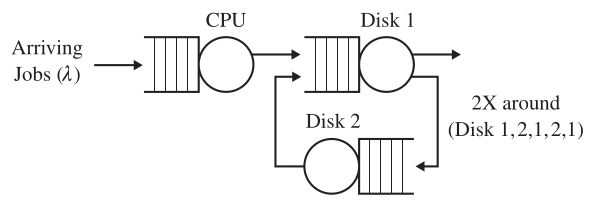
\includegraphics[width=0.65\linewidth]{images/open_network.jpg}
        \caption{An open queueing network}
    \end{figure}
\end{frame}

% \note{
%     Note 1
% }

\section{Jackson Network}

\begin{frame}
    \frametitle{Jackson Network}
    \begin{itemize}
        \item General form of queueing network
        \begin{itemize}
            \item Unbounded queues
            \item FCFS (First Come First Serve) service
            \item Arrivals from outside network \(\sim\) Poisson(\(r_i\))
            \item Service rates \(\sim\) exp(\(\mu_i\))
            \item Probabilistic routing - \(P_{ij}\)
            \item States: \((n_1, n_2, \ldots, n_k)\)
            $$ \lambda_i = r_i + \sum_j \lambda_j P_{ji} \quad \text{.} $$
        
        \end{itemize}
    \end{itemize}
        \begin{figure}
        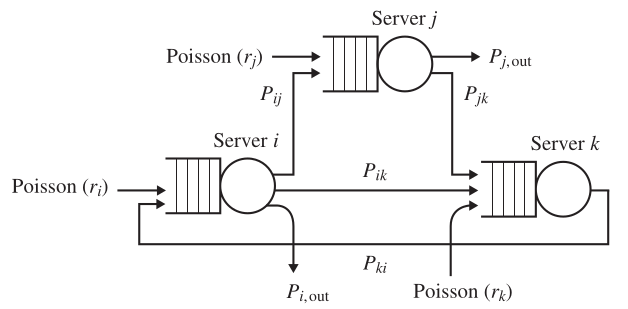
\includegraphics[width=0.65\linewidth]{images/jackson_network.jpg}
        \caption{A Jackson network}
    \end{figure}
\end{frame}

\begin{frame}
    \frametitle{Independency?}
        \begin{itemize}
            \item Consider a single server network with properties:
            \begin{itemize}
                \item Low arrival rate
                \item High service rate
                \item High \(P_{ii}\)
            \end{itemize}
        \end{itemize}
        \begin{figure}
            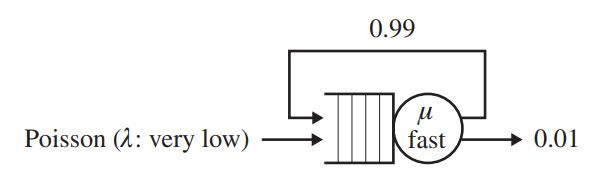
\includegraphics[width=0.65\linewidth]{images/independency_network.jpg}
        \end{figure}
        \begin{center} 
            Incremental increments property unsatisfied
        \end{center}

\end{frame}

\begin{frame}
    \frametitle{Solving the Jackson}
    \begin{center} 
    \linespread{1.6}
        Rate of jobs leaving the state = Rate entering the state
   \[
\pi_{n_1,n_2,\ldots,n_k} \cdot \left[ \sum_{i=1}^{k} r_i + \sum_{i=1}^{k} \mu_i (1 - P_{ii})  \right] = 
\]
        \begin{equation}
\begin{aligned}
    \notag
    &\underbrace{\sum_{i=1}^{k} \pi_{n_1,\ldots,n_i - 1,\ldots,n_k} \cdot r_i}_{\text{outside arrival}}
    + \underbrace{\sum_{i=1}^{k} \pi_{n_1,\ldots,n_i + 1,\ldots,n_k} \cdot \mu_i P_{i,\text{out}}}_{\text{departure to outside}} \\
    &+ \underbrace{\sum_{i=1}^{k} \sum_{j \neq i} \pi_{n_1,\ldots,n_i - 1,\ldots,n_j + 1,\ldots,n_k} \cdot \mu_j P_{ji}}_{\text{internal transition from server } j \text{ to server } i, j \neq i}.
\end{aligned}
\end{equation}

        
    \end{center}
    

\end{frame}

\begin{frame}
    \frametitle{Solving the Jackson(contd.)}
    \begin{itemize}
        \item Very hard to solve
        \item Is there no better method?
        \item Local Balance Approach
        \begin{itemize}
            \item No exact algorithm
            \item Part of setting up equations is the "art"
            \item Break both sides of the equation into k+1 matching components and then equate
            \item First component - Outside arrivals/departures
        \end{itemize}
    \end{itemize}
    \begin{center} 
    Rate leaving state due to outside arrival =
    Rate entering state due to outside departure 
                
    \end{center}
    
\end{frame}

\begin{frame}
    \frametitle{Solving the Jackson(contd.)}
    \begin{center} 
        A = A'
        \[\sum_{i=1}^{k} \pi_{n_1,\ldots,n_i,\ldots,n_k} r_i = \sum_{i=1}^{k} \pi_{n_1,\ldots,n_i+1,\ldots,n_k} \mu_i P_{i,\text{out}}\]
    \end{center}
        \begin{itemize}
        \item Can we make a guess for \(\pi_{n_1,\ldots,n_k}\) such that it satisfies the above equality?
        \item Observe that \(\pi_{n_1,\ldots,n_i,\ldots,n_k}\) term in A and the \(\pi_{n_1,\ldots,n_i+1,\ldots,n_k}\) term in A' only differ in the \(n_i\) spot
        \item Let 
    \end{itemize}
    
    \begin{center} 
        \(\pi_{n_1,\ldots,n_i,\ldots,n_k} \cdot c_i = \pi_{n_1,\ldots,n_i+1,\ldots,n_k}\)
    \end{center}
\end{frame}

\begin{frame}
    \frametitle{Solving the Jackson(contd.)}
        \[
        \sum_{i=1}^{k} \pi_{n_1,\ldots,n_i,\ldots,n_k} r_i = \sum_{i=1}^{k} \pi_{n_1,\ldots,n_i+1,\ldots,n_k} \mu_i P_{i,\text{out}}
        \]
        \[
        \sum_{i=1}^{k} \pi_{n_1,\ldots,n_i,\ldots,n_k} r_i = \sum_{i=1}^{k} \pi_{n_1,\ldots,n_k} \cdot c_i \cdot \mu_i P_{i,\text{out}}
        \]
        \[
        \sum_{i=1}^{k} r_i = \sum_{i=1}^{k} (c_i \cdot \mu_i) P_{i,\text{out}}.
        \]

    
\end{frame}
\begin{frame}
    \frametitle{Solving the Jackson(contd.)}
    Observe that if:
    \[c_i \cdot \mu_i = \lambda_i\]
    Then:
    \[\sum_{i=1}^{k} r_i = \sum_{i=1}^{k} \lambda_i P_{i,\text{out}}.\] \[c_i = \frac{\lambda_i}{\mu_i} = \rho_i\]
    Now,
    \[\pi_{n_1}, \ldots, \pi_{n_i}, \ldots, \pi_{n_k} \cdot \rho_i = \pi_{n_1}, \ldots, \pi_{n_i+1}, \ldots, \pi_{n_k} \quad \forall i\]
    
\end{frame}

\begin{frame}
    \frametitle{Solving the Jackson(contd.)}
    Hence, it is reasonable to assume that:
    \[\pi_{n_1}, \ldots, \pi_{n_i}, \ldots, \pi_{n_k} = C \rho_{n_1}^{1} \ldots \rho_{n_k}^{k}\]
    where C is the normalizing constant. Now we will solve for:
    \[B_i = B_i'\]
    Here, \(B_i\) is the rate of rate of transitions leaving state \((n_1, n_2, \ldots, n_k)\) due to a departure from server i. Hence,
    \[B_i = \pi_{n1}, \ldots, \pi_{nk} \cdot \mu_i(1 - P_{ii}).\]
\end{frame}

\begin{frame}
    \frametitle{Solving the Jackson(contd.)}
    And \(B_i'\) is the rate of transitions entering \((n_1, n_2, \ldots, n_k)\) due to an arrival at server i. Hence,
    \[
        B'_i = \underbrace{\sum_{\substack{j \text{ s.t. } j \neq i}} \pi_{n_1,\ldots,n_i-1,\ldots,n_j+1,\ldots,n_k} \mu_j P_{ji}}_{\text{internal transition from server } j \text{ to server } i (j \neq i)} + \underbrace{\pi_{n_1,\ldots,n_i-1,\ldots,n_k} r_i}_{\text{outside arrival}}.
    \]
    Now, we will put:
    \[\pi_{n_1}, \ldots, \pi_{n_i}, \ldots, \pi_{n_k} = C \rho_{n_1}^{1} \ldots \rho_{n_k}^{k}\]

\end{frame}

\begin{frame}
    \frametitle{Solving the Jackson(contd.)}
    \begin{align*}
        B_i &= B'_i \\
        C \rho_1^{n_1} \rho_2^{n_2} \cdots \rho_k^{n_k} \mu_i (1 - P_{ii}) &= \sum_{j \neq i} C \rho_1^{n_1} \rho_2^{n_2} \cdots \rho_k^{n_k} \left( \frac{\rho_j}{\rho_i} \right) \mu_j P_{ji} \\
        &\phantom{=} + C \rho_1^{n_1} \rho_2^{n_2} \cdots \rho_k^{n_k} \left( \frac{1}{\rho_i} \right) r_i \\
        \mu_i (1 - P_{ii}) &= \sum_{j \neq i} \frac{\rho_j \mu_j P_{ji}}{\rho_i} + \frac{r_i}{\rho_i} \\
        \rho_i \mu_i (1 - P_{ii}) &= \sum_{j \neq i} \rho_j \mu_j P_{ji} + r_i \\
        \lambda_i (1 - P_{ii}) &= \sum_{j \neq i} \lambda_j P_{ji} + r_i
    \end{align*}

\end{frame}

\begin{frame}
    \frametitle{Solving the Jackson(contd.)}
    Lastly, we need to find the normalizing constant \( C \):

    \[
    \sum_{n_1,\ldots,n_k} \pi_{n_1,\ldots,n_k} = 1
    \]
    
    \[
    C \sum_{n_1,\ldots,n_k} \rho_1^{n_1} \cdots \rho_k^{n_k} = 1
    \]
    
    \[
    C \left( \sum_{n_1} \rho_1^{n_1} \right) \left( \sum_{n_2} \rho_2^{n_2} \right) \cdots \left( \sum_{n_k} \rho_k^{n_k} \right) = 1
    \]
    
    \[
    C \left( \frac{1}{1 - \rho_1} \right) \left( \frac{1}{1 - \rho_2} \right) \cdots \left( \frac{1}{1 - \rho_k} \right) = 1
    \]
    
\end{frame}

\begin{frame}
    \frametitle{Solving the Jackson(contd.)}
    Hence,
    
    \[
    C = (1 - \rho_1) (1 - \rho_2) \cdots (1 - \rho_k).
    \]
    As a result,
    
    \[
    \pi_{n_1,\ldots,n_k} = \rho_1^{n_1} (1 - \rho_1) \rho_2^{n_2} (1 - \rho_2) \cdots \rho_k^{n_k} (1 - \rho_k).
    \]

    
    Now, what about the jobs at server i?
    For server 1:
    \[
    P\{n_1 \text{ jobs at server } 1\} = \sum_{n_2,\ldots,n_k} \pi_{n_1,\ldots,n_k}
    \]
    
\end{frame}

\begin{frame}
    \frametitle{Solving the Jackson(contd.)}
    \[
    = \sum_{n_2,\ldots,n_k} \rho_1^{n_1} (1 - \rho_1) \rho_2^{n_2} (1 - \rho_2) \cdots \rho_k^{n_k} (1 - \rho_k) = \rho_1^{n_1} (1 - \rho_1).
    \]
    
    Likewise,
    
    \[
    P\{n_i \text{ jobs at server } i\} = \rho_i^{n_i} (1 - \rho_i).
    \]
    Which means that all servers behave like M/M/1 queues in terms of their stationary queue length distributions even though their arrival processes are not usually Poisson.
\end{frame}

\end{document}
